\section{Semaine 01 (16/09-20/09) }


\e{Notions abordées :}
\begin{itemize}
	\item Analyse dimensionnelle.
	\item Circuits électriques dans l'ARQS.
\end{itemize}


\subsection{Questions de cours}

\begin{enumerate}
	\item Définir le courant électrique. Définir l'intensité du courant électrique.
	\item Définir la tension électrique.
	\item Décrire les conventions d'orientation des dipôles. Que valent la puissance reçues et fournies dans chaque cas ?
	\item Qu'est-ce que l'ARQS ? Quelles conséquences ?
	\item Démontrer la formule du pont diviseur de tension.
	\item Démontrer la formule du pont diviseur de courant.
\end{enumerate}

\subsection{Exercice 1 : Application des lois de Kirchoff}

Pour chaque circuit, donner les tensions $u$ et $u_1$ en fonction de $e$ ou bien les intensités $i$ et $i_1$ en fonction de $i_0$.

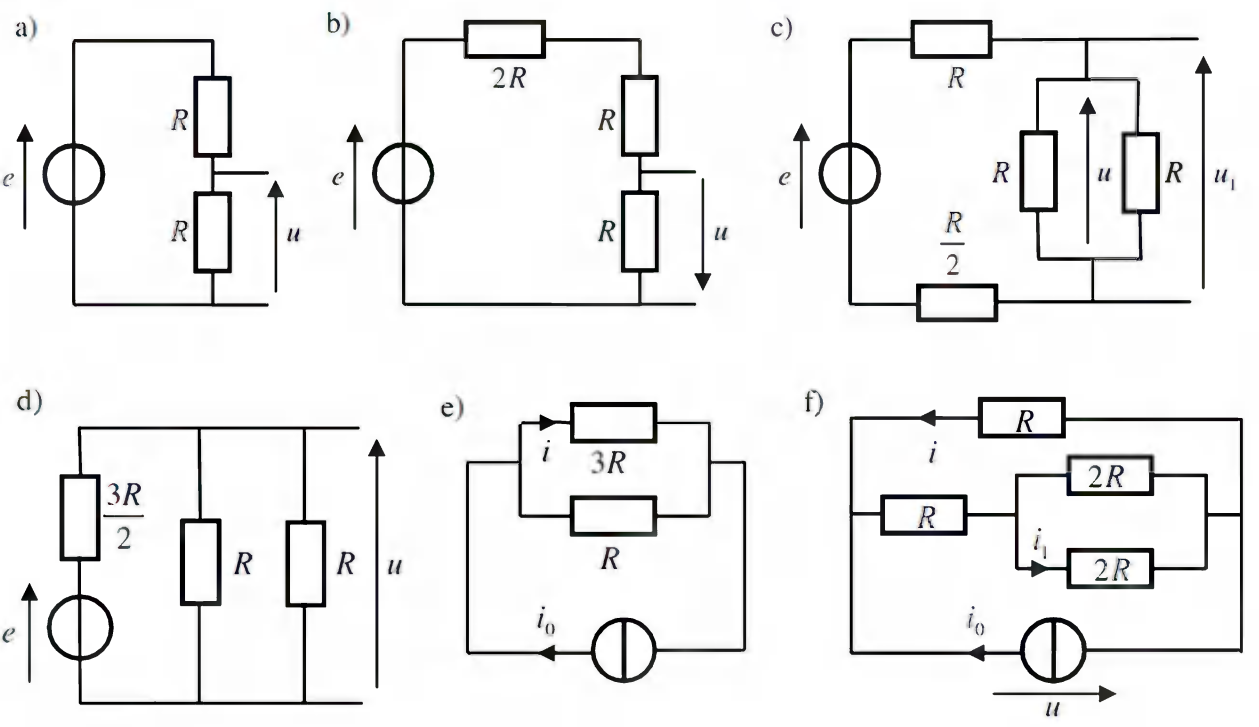
\includegraphics[width=\textwidth]{Images/exercicesKirchoff.png}

\subsection{Exercice 2}

\begin{minipage}[c]{\linewidth/2}
	\begin{circuitikz}
		%Circuit
		\draw (4, 0)
			to[short, i>=$I$] (2, 0)
			to[R, l=$R$] (0, 0)
			to[vsource, v_<=$e$] (0, -3)
			-- (4, -3);
		\draw (2, 0)
			to[R, l_=$R$, v^<=$U$] (2, -3);
	\end{circuitikz}
\end{minipage}%
\begin{minipage}[c]{\linewidth/2}
	On donne $R = \SI{10}{k\Omega}$.
	\begin{enumerate}
		\item Tracer la caractéristique du dipôle ci-contre.
		\item On ajoute une charge de résistance $R'=\SI{3}{k\Omega}$. Déterminer le point de fonctionnement de deux façons.
	\end{enumerate}
\end{minipage}

\subsection{Exercice 3 : Rendement d'un montage potentiométrique}

\begin{minipage}[c]{\linewidth/2}
	\begin{circuitikz}
		%Circuit
		\draw (0, 2)
		to[short, i>=$I$] (0, 3)
		--++(2, 0)
		to[R, l=$r_2$] ++(0, -2)
		to[R, l=$r_1$] ++(0, -2)
		--++(-2, 0)
		--++(0, 1)
		to[vsource, v=$E$] (0, 2);
		\draw (2, 1)
		to[short, i=$i_R$] ++(2, 0)
		to[R, l=$R$] ++(0, -2)
		--++(-2, 0);
	\end{circuitikz}
\end{minipage}%
\begin{minipage}[c]{\linewidth/2}
	Le rendement $\eta$ de ce diviseur de tension est le rapport $P_R$ de la puissance dissipée dans la résistance de charge $R$ à la puissance $P_E$ fournie par la source de tension $E$. Exprimer $\eta$ en fonction de $r_1$, $r_2$ et $R$.
	
	AN : $r_1 = \SI{750}{\Omega}$, $r_2=\SI{250}{\Omega}$, $R = \SI{80}{\Omega}$. Commentaire.
\end{minipage}

\subsection{Exercice 4 : Adaptation de puissance}

\begin{minipage}[c]{\linewidth/2}
	\begin{circuitikz}
		%Circuit
		\draw (0, 0)
		to[R, l=$R_0$] (3, 0)
		to[R, l=$R$] (3, -3)
		-- (0, -3)
		to[vsource, v=$E$] (0, 0);
	\end{circuitikz}
\end{minipage}%
\begin{minipage}[c]{\linewidth/2}
	Un générateur présente une tension à vide $E$ et une résistance interne $R_0$. On y branche une charge de résistance $R$. Pour quelle valeur de $R$ la puissance dissipée dans la résistance $R$ est elle maximale ? Que vaut alors cette puissance ?
\end{minipage}
